
We present the results on two sets of experiments on synthetic data.

\subsection{Deblending two stars}

We set up a simple experiment to study the
ability of StarNet to deblend two stars.
On a $20\times20$ pixel image,
we simulate two stars of equal flux at distance $\delta$ pixels apart, and
examine the approximate posterior produced by StarNet (Figure~\ref{fig:deblending_fig}).
When stars are separated by 1.5 pixels, StarNet assigns nearly 100\% probability
of two stars in the image.

\begin{figure}[tb]
    \centering
    \begin{subfigure}{0.8\textwidth}
        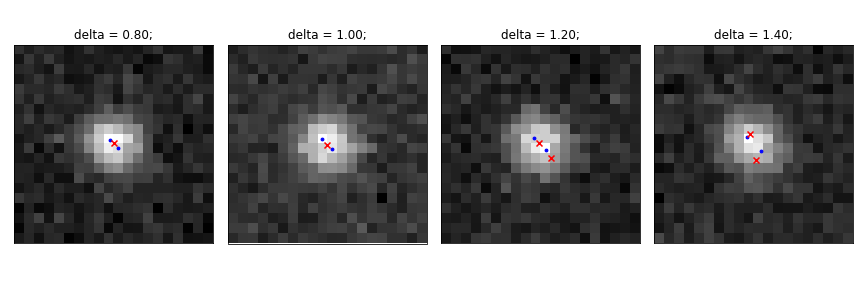
\includegraphics[width=\textwidth]{figures/deblending/example_deblending.png}
    \end{subfigure}
    \begin{subfigure}{0.8\textwidth}
        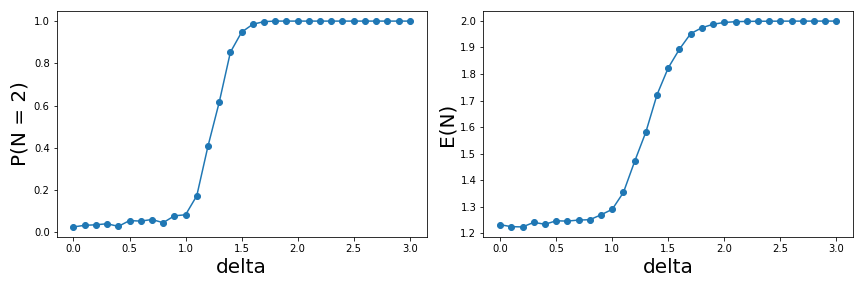
\includegraphics[width=\textwidth]{figures/deblending/summary_statistics.png}
    \end{subfigure}
    \caption{(Top row) Simulated images with two stars separated by distance $\delta$ in pixels.
    True locations are in blue. Red are detections from the starnet MAP estimate.
    In these examples, Starnet correctly identified the two stars separated by distance $\delta \geq 1.2$,
    but only estimated one star when $\delta \leq 1$.
    (Bottom left) The probability that $N$, the number of sources in the image, equals two
    under the variational posterior, as $\delta$ varies.
    (Bottom right) The expectation of $N$ under the variational posterior as $\delta$ varies. }
    \label{fig:deblending_fig}
\end{figure}

\subsection{Coverage of credible intervals}

We have seen that on M2, the StarNet 95\% credible interval failed
to contain the ground truth number of stars (Section~\ref{sec:results_on_m2}).
On M2, we attribute this to model mis-specification, specifically due to a poorly
estimated background.

We check the coverage of StarNet credible intervals on synthetic data
to rule out any issues with model mis-specification.
On synthetic data, StarNet again overestimates the number of stars.
On a single simulated image sampled from the prior,
the true number of stars ($N = 1195$),
is still considerably smaller than the 0.01-th percentile of
the approximate posterior distribution (Figure~\ref{fig:starnet_density}).


\begin{figure}[tb]
    \centering
    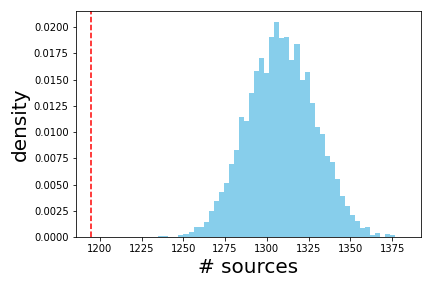
\includegraphics[width=0.6\textwidth]{./figures/coverage/starnet_histogram.png}
    \vspace{-0.4cm}
    \caption{Distribution of 5000 samples of the number of sources from the starnet approximate posterior.
    The true number of sources demarcated in red. }
    \label{fig:starnet_density}
\end{figure}

We attribute this over-estimation due to the spatial independence of the apprximate posterior.
Specifically, StarNet \textit{overestimates} the number of sources close to tile boundaries.
Heuristically, for a tile containing
a source located in the interior of the tile
within $\epsilon$ of a boundary (but still far from a corner),
StarNet should assign a probability of $\frac{1}{2}$ for
having one source, and a probability $\frac{1}{2}$ for having none, as $\epsilon \rightarrow 0$.
Should this be the case, then over the entire image, which consist of many tiles,
a source on the edge is correctly accounted for: it has a 50-50 chance of being assigned to one tile or another
in the approximate posterior, and the expected number of sources sum to one.

However, we observe empirically that as a source approaches the edge of a tile,
the probability that $N = 1$ approaches a number
slightly \textit{larger} than $\frac{1}{2}$ (Figure~\ref{fig:starnet_edges}).
Therefore, the approximate posterior overestimates the expected number of sources in the full entire image.
If we were to simulate images with the constraint that sources are at least 0.1-pixels from the edge,
then the StarNet approximate posterior has much closer to correct coverage (Figure~\ref{fig:coverage_good})

\begin{figure}[tb]
    \centering
    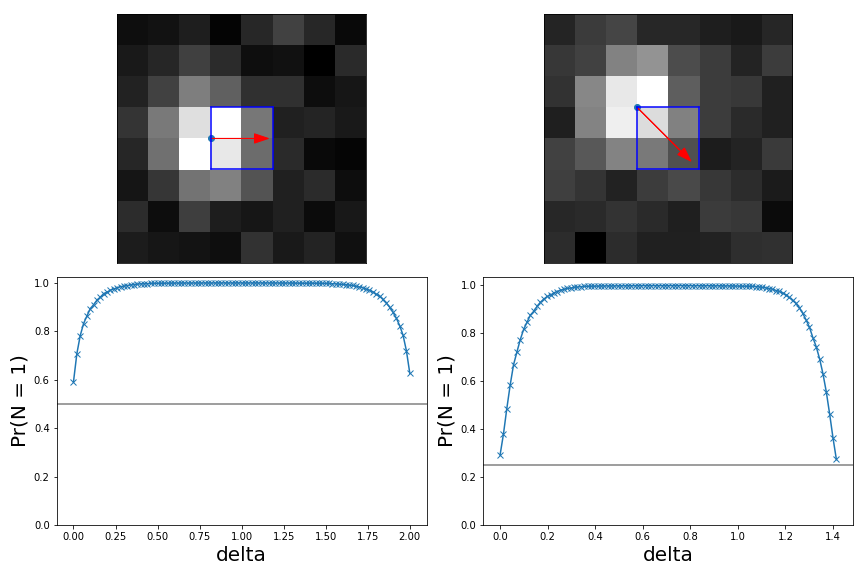
\includegraphics[width=0.8\textwidth]{./figures/coverage/edges_example.png}
    \vspace{-0.4cm}
    \caption{The expected number of sources under the starnet approximate posterior as a function of distance from the edge (in pixels).
    On the left, we place a star on the left-most edge, and move its location $\delta$ pixels to the right.
    On the right, we place a star on the top-left corner, and move its location $\delta$ pixels towards the bottom-right corner.}
    \label{fig:starnet_edges}
\end{figure}

\begin{figure}[tb]
    \centering
    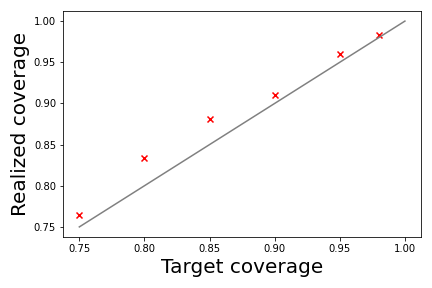
\includegraphics[width=0.8\textwidth]{./figures/coverage/good_coverage.png}
    \vspace{-0.4cm}
    \caption{Coverage test in simulated $100\times100$ images where all true stars are constrained to be 0.1-pixels away from any tile
    boundary.
    We simulate 1000 images from the prior and generative model, and for each image, we compute a $1 - \alpha$-level credible
    interval for the number of stars by taking the $\alpha/2$ and $1 -\alpha/2$-th percentiles of StarNet 5000 samples.
    For each $\alpha$, we plot the observed coverage against the target $1 - \alpha$-level coverage. }
    \label{fig:coverage_good}
\end{figure}
